\documentclass[handout]{beamer}

%\usepackage[table]{xcolor}
\mode<presentation> {
  \usetheme{Boadilla}

%  \usetheme{Pittsburgh}
%\usefonttheme[2]{sans}
\renewcommand{\familydefault}{cmss}
%\usepackage{lmodern}
%\usepackage[T1]{fontenc}
%\usepackage{palatino}
%\usepackage{cmbright}
%  \setbeamercovered{transparent}
\useinnertheme{rectangles}
}

\setbeamercolor{normal text}{fg=black}
\setbeamercolor{structure}{fg= blue}
\definecolor{trial}{cmyk}{1,0,0, 0}
\definecolor{trial2}{cmyk}{0.00,0,1, 0}
\definecolor{darkgreen}{rgb}{0,.4, 0.1}
\usepackage{array}
\beamertemplatesolidbackgroundcolor{white}  \setbeamercolor{alerted
text}{fg=red}
\usepackage{tcolorbox}
\setbeamertemplate{caption}[numbered]\newcounter{mylastframe}

\font\domino=domino
\def\die#1{{\domino#1}}
\usepackage{tikz}
\usetikzlibrary{arrows}
\usepackage{colortbl}

\renewcommand{\familydefault}{cmss}
%\usepackage[all]{xy}

\usepackage{tikz}
\usepackage{lipsum}

 \newenvironment{changemargin}[3]{%
 \begin{list}{}{%
 \setlength{\topsep}{0pt}%
 \setlength{\leftmargin}{#1}%
 \setlength{\rightmargin}{#2}%
 \setlength{\topmargin}{#3}%
 \setlength{\listparindent}{\parindent}%
 \setlength{\itemindent}{\parindent}%
 \setlength{\parsep}{\parskip}%
 }%
\item[]}{\end{list}}
\usetikzlibrary{arrows}

\usecolortheme{lily}

\newtheorem{com}{Comment}
\newtheorem{lem} {Lemma}
\newtheorem{prop}{Proposition}
\newtheorem{condition}{Condition}
\newtheorem{thm}{Theorem}
\newtheorem{defn}{Definition}
\newtheorem{cor}{Corollary}
\newtheorem{obs}{Observation}
\numberwithin{equation}{section}
 

\setbeamertemplate{navigation symbols}{}


\title[PLSC 43401]{Mathematical Foundations of Political Methodology}

\author{Robert Gulotty}
\institute[Chicago]{University of Chicago}
\vspace{0.3in}




\begin{document}

\begin{frame}
\maketitle
\end{frame}


\begin{frame}
\frametitle{Day 3: Random Variables: Discrete}

\begin{itemize}
\item Random Variables
\item Expectation, Variance
\item Discrete Probability Mass Function
\item Cumulative Distribution Functions
\item Joint Probability Mass Functions
\end{itemize}
\end{frame}


\begin{frame}
\frametitle{Random Variables}
Given a sample space $\Omega$, and a probability law $P$:
\begin{defn}
A \emph{random variable} is a \alert{function} that assigns real numbers (usually) to events in a sample space $\Omega$.
\end{defn}
$$X(\omega): \Omega \to \mathbb{R}$$

\end{frame}



\begin{frame}
\frametitle{Random Variables: Example}
Sample space from tossing three coins: 

$$\Omega=\{ HHH,\ HHT,\ HTH,\ THH,\ HTT,\ THT,\ TTH,\ TTT\}$$

Let $Y(\omega)$ be the number of heads in outcome $\omega \in \Omega$.\pause

\begin{itemize}
\item $Y(HHH)=3$\pause
\item $Y(HHT)=Y(HTH)=Y(THH)=2$\pause
\item $Y(HTT)= Y(THT)=Y(TTH)=1$\pause
\item $Y(TTT)=0$
\end{itemize}
\end{frame}

\begin{frame}
\frametitle{Random Variables: Example II}
Sample space from the number of dots on a die roll.

\quad $\Omega=\{$\die1,\die2,\die3,\die4,\die5,\die6$\}$

Let $Z(\omega)$ be the dots on the die face $\omega \in \Omega$.\pause

\begin{itemize}
\item Z(\die1)=1
\item Z(\die2)=2
\item Z(\die3)= 3
\item Z(\die4)=4
\item Z(\die5)=5
\item Z(\die6)=6
\end{itemize}
\end{frame}

\begin{frame}
\frametitle{Random Variables: Example III}
Sample space from the number of dots on a die roll.

\quad $\Omega=\{$\die1,\die2,\die3,\die4,\die5,\die6$\}$

Let $X(\omega)$ be 3 to the power of the number of dots on the die face $\omega \in \Omega$ minus 1.\pause

\begin{itemize}
\item X(\die1)$=3^{1-1}$\pause$=3^0=1$\pause
\item X(\die2)$=3^{2-1} = 3$
\item X(\die3)$=3^{3-1} = 9$
\item X(\die4)$=3^{4-1} = 27$
\item X(\die5)$=3^{5-1} = 81$
\item X(\die6)$=3^{6-1} =  243$
\end{itemize}
\pause
$X(\omega)=3^{\omega-1}$
\end{frame}


\begin{frame}[fragile]{functions}
\begin{itemize}
\item Random Variables are functions.
\item In R, we see functions look like a word followed by ():
\begin{itemize}
\item mean(), median(), head(), str()
\end{itemize}
\item Our own functions are written using:
\end{itemize}
 
\begin{verbatim}
 function(input){ 
     do something 
     return(output)}
 \end{verbatim}

\end{frame}

\begin{frame}
\frametitle{Properties of Random Variables}

Random variables (for us) will always give a number.
\begin{itemize}
\item X,Y, Z: capital letters for a random variable.
\item x, y, z: are the output of the function.
\end{itemize}
\end{frame}


\begin{frame}
\frametitle{Kinds of Random Variables}
\begin{defn}
A random variable may be 
\begin{enumerate}
\item discrete: if outcomes are countable.
\item continuous: If outcomes can be any value in some interval.
\item mixed: if outcomes are a combination of events and intervals.
\end{enumerate}
\end{defn}
\end{frame}


\begin{frame}
\frametitle{Connecting random variables to probability}
\begin{itemize}
\item X assigns some numbers to events.\pause
\item Remember, probability assigns a likelihood to an event.\pause
\item What is the probability that $X(\omega)$ gives some number x?\pause
\item $P(X=x)\pause $$ \equiv P(\{\omega \in \Omega : X(\omega)= x\})$
\item This is another function (of a function)
\end{itemize}
\end{frame}


\begin{frame}
\frametitle{Discrete Probability Function}
\begin{defn}

If X is a discrete random variable, the probability of each outcome x is provided by a probability function:
$$p_X(x)=P(X=x)=P(\{\omega \in \Omega: X(\omega)=x\})$$

\end{defn}
\begin{itemize}
\item this is also called the \emph{probability mass function} (pmf)
\item We often just write $p(x)$, some people use $f_X(x)$
\end{itemize}

\end{frame}

\begin{frame}
\frametitle{Building a Discrete Probability Function: Example}
\begin{itemize}
\item Sample space: $\Omega= \{\text{Pashto, Not Pashto}\}$
\item X=1 if $\omega=\text{Pashto}$
\item X=0 if $\omega=\text{Not Pashto}$ 
\item P(X=1)=.3
\end{itemize}
A pmf can take on any value of x, so we must consider all possibilities of x.
\begin{itemize}
\item $x = 1$
\item $x = 0$
\item all other values of x.
\end{itemize}
\end{frame}


\begin{frame}
\begin{itemize}
\item If $x = 1$
$$P(X=x)=P(X=1)=P(\text{Pashto})=p=.3$$\pause
\item If $x = 0$
$$P(X=x)=P(X=0)=P(\text{Not Pashto})=1-p=.7$$\pause
\item all other values of x.
$$P(X=x)=0$$
\end{itemize}\pause
Combining these results, we get the probability function.

$$f_X(x)=\begin{cases}
p & \text{if}\ x=1\\
1-p & \text{if}\ x=0\\
0 & \text{otherwise}
\end{cases}$$\pause
This can be written shorthand as:
$$f_X(x)=p^x(1-p)^{(1-x)},\ \ x\in \{0,1\}$$ 
Where the 0 is left implicit.

\end{frame}



\begin{frame}
\frametitle{Dichotomous process}

To summarize
\begin{itemize}
\item If X only has two values $0$ and $1$ and $p=P(X=1)$
\item[] then $X$ has the probability function:
$$f_X(x)=p^x(1-p)^{(1-x)},\ \ x\in \{0,1\}$$
\pause
\item This is called a Bernoulli distribution:
$$X\sim \text{Bernoulli}(p)$$
\item $p$ is a \emph{parameter}
\end{itemize}
\end{frame}



\begin{frame}
\frametitle{Bernoulli Random Variable}

Suppose we flip a fair coin and $Y = 1$ if the outcome is Heads . \\

\begin{eqnarray}
Y & \sim & \text{Bernoulli}(1/2) \nonumber \\
p(1) & = & (1/2)^{1} (1- 1/2)^{ 1- 1} = 1/2 \nonumber \\
p(0) & = & (1/2)^{0} (1- 1/2)^{1 - 0} = (1- 1/2) \nonumber 
\end{eqnarray}



\end{frame}


\begin{frame}
\frametitle{Example: Winning a War}

Suppose country $1$ is engaged in a conflict and can either win or lose. \pause  \\
Define $Y = 1$ if the country wins and $Y = 0$ otherwise.\\ \pause 
Then,  \pause 
\begin{eqnarray}
Y &\sim & \text{Bernoulli}(\pi) \nonumber \pause 
\end{eqnarray}


Suppose country $1$ is deciding whether to fight a war.  \\\pause 
Engaging in the war will cost the country $c$.  \\ \pause 
If they win, country $1$ receives $B$.  \\ \pause 
What is $1$'s expected utility from fighting a war?\\ \pause 
\begin{eqnarray}
E[U(\text{war})] & = & (\text{Utility}|\text{win})\times P(\text{win}) + (\text{Utility}| \text{lose})\times P(\text{lose}) \nonumber \\ \pause 
&= & (B - c) P(Y = 1) + (- c) P(Y = 0 )\nonumber \\ \pause 
& = & B \times p(Y = 1)  - c(P(Y = 1)  + P(Y = 0)) \nonumber \\ \pause 
& = & B \times \pi - c \nonumber 
\end{eqnarray}
\pause 

\end{frame}

\begin{frame}
\frametitle{Example: Sequence of Bernoulli trials}

We might be interested in the outcome of several independent trials \textbf{ie. with replacement}.\\
\pause
Consider a coin, flipped twice.  Suppose $X_1(T)=0$, $X_1(H)=1$, $X_2(T)=0$, $X_2(H)=1$  \pause
$$P(X_1=1,\ X_2=1)=P(X_1=1\cap X_2=1)= P(X_1=1)P(X_2=1) $$
\pause
$$p(x_1, x_2)= p^{x_1}(1-p)^{1-x_1}p^{x_2}(1-p)^{1-x_2}$$
\pause
$$p(x_1, x_2)= p^{x_1+x_2}(1-p)^{2- x_1- x_2}$$
\pause
Let $X_1,...,\ X_n$ be independent Bernoulli random variables with the same parameter $p$.
$$p(x_1,...x_n)=p(x_1)p(x_2)... p(x_n)= p^{x_1+...x_n}(1-p)^{n-x_1-....-x_n}$$
$$\ \ \text{for}\ x_i\in\{0,1\} \ \text{and}\ i=1,...,n$$

\end{frame}


\begin{frame}
\frametitle{Expectation}

What can we \alert{expect} from a trial? \pause \\

Value of random variable for any outcome weighted by the probability of observing that outcome \pause \\
probability weighted average \pause \\

\begin{defn} 
Expected Value: define the expected value of a function $X$ as, 
\begin{eqnarray}
E[X] &  = & \sum_{x:p(x)>0} x p(x) \nonumber \pause 
\end{eqnarray}
In words: for all values of $x$ with $p(x)$ greater than zero, take the weighted average of the values
\end{defn} 

\end{frame}


\begin{frame}
\frametitle{Expectation informally}

The expectation is based on the principle that the value of a future gain should be directly proportional to the chance of getting it.

$$E[X+Y]=E[X]+E[Y]$$
$$E[a]=a$$
$$E[aX]=aE[X]$$
$$E[E[X]]=E[X]$$

$$E[XY]\neq E[X]\times E[Y]$$

\end{frame}


\begin{frame}
\frametitle{Properties of the Expecation}
$$E[a]=a$$\pause 
Proof:  Suppose Y is a random variable = a with probability 1 and 0 otherwise:
$$E[Y] = \sum_{y: p(y)>0} y p(y) = a * 1 $$  \pause 

Also: 
$$E[aX] = \sum_{x: p(x)>0} a\ x\  p(x) $$  \pause 
$$E[aX] = a \sum_{x: p(x)>0} x\  p(x) $$  \pause
\end{frame}


\begin{frame}
\frametitle{Indicator Variables and Probabilities} 

\pause 
\begin{prop}\pause 
Suppose $A$ is an event.  Define random variable $I$ such that $I= 1$ if an outcome in $A$ occurs and $I =0$ if an outcome in $A^{c}$ occurs.  Then,  \pause 
\begin{eqnarray}
E[I] &  = &  P(A)\nonumber  \pause 
\end{eqnarray}

\begin{proof}  \pause 
\begin{eqnarray}
E[I]  & =&  1 \times P(A) + 0 \times P(A^{c}) \nonumber \\ \pause 
 & = & P(A) \nonumber 
\end{eqnarray} 
\end{proof}


\end{prop}

\end{frame}






\begin{frame}
\frametitle{Variance} 

Expected value is a measure of \alert{central tendency}. \pause \\
What about spread? \pause  \alert{Variance}  \pause \\
\begin{itemize}
\item[-] For each value, we might measure distance from center \pause 
\begin{itemize}
\item[-] Euclidean distance, squared $d(x, E[x])^{2} = (x - E[x])^2$  \pause 
\end{itemize}
\item[-] Then, we might take weighted average of these distances,  \pause 
\tiny{
\begin{eqnarray} 
E[(X - E[X])^2] & = & \sum_{x} (x  - E[X])^2p(x) \nonumber \\  \pause 
& = & \sum_{x} \left(x^2  -E[X] x -x E[X] + E[X]^2\right) p(x) \nonumber \\  \pause 
& = & \sum_{x} x^2 p(x)   - \sum_{x} 2x E[X]p(x) + \sum_{x} E[X]^2 p(x) \nonumber \\  \pause 
& = & \sum_{x} x^2 p(x)   - 2E[X] \sum_{x} x p(x) + \sum_{x} E[X]^2 p(x) \nonumber \\  \pause 
&  = &  E[X^2] - 2E[X]^2 + E[X]^2  \nonumber \\ \pause 
& = & E[X^2] - E[X]^2 \nonumber \\ \pause 
& = & \text{Var}(X) \nonumber 
\end{eqnarray}
}
\end{itemize}

\end{frame}


\begin{frame}
\frametitle{Variance}

\begin{defn}
The variance of a random variable $X$, var$(X)$, is 
\begin{eqnarray}
 \text{var}(X) & = & E[(X - E[X])^2] \nonumber \\
 & = &  E[X^2] - E[X]^2 \nonumber 
\end{eqnarray}
\end{defn}

\begin{itemize}
\item[-] We will define the standard deviation of $X$, sd$(X) = \sqrt{\text{var}(X)} $
\item[-] var$(X) \geq 0$.  
\end{itemize}


\end{frame}




\begin{frame}
\frametitle{Variance Corollary} 

\begin{cor}
Var($aX  + b$)  = $a^2$Var($X$) 
\end{cor} 
\pause 
\begin{proof} 
Define $Y = aX +b$.  Now, we know that \\ \pause 
$Var(Y) = E[(Y - E[Y])^2]$.  Let's substitute and use our other corollary \pause 
\begin{eqnarray}
Var(Y) & =& E[ (aX + b - a E[X] - b)^2 ] \nonumber  \pause \\
 & = & E[ (a^2 X^2 - 2 a^2 X E[X] + a^2 E[X]^2)] \nonumber  \pause \\
& = & a^2E[X^2] -2a^2E[X]^2 + a^2 E[X]^2 \nonumber  \pause \\
& = & a^2(E[X^2] - E[X]^2) \nonumber \pause  \\
 & = & a^2 Var(X) \nonumber 
 \end{eqnarray}
\end{proof} 

\end{frame}


\begin{frame}
\frametitle{Bernoulli Random Variable \alert{Moments}}
Suppose $Y \sim \text{Bernoulli}(\pi)$ \\


\begin{eqnarray} 
E[Y] & = & 1 \times P(Y = 1) + 0 \times P(Y = 0) \nonumber \\
& = & \pi + 0 (1 - \pi) \nonumber  = \pi  \nonumber \\
\text{var}(Y) & = & E[Y^2] - E[Y]^2 \nonumber  \\
E[Y^2] & = & 1^{2} P(Y = 1) + 0^{2} P(Y = 0) \nonumber \\
& = & \pi \nonumber \\ 
\text{var}(Y) & = & \pi - \pi^{2} \nonumber \\
& = & \pi(1 - \pi ) \nonumber 
\end{eqnarray}

$E[Y] = \pi$\\
var$(Y) = \pi(1- \pi) $
What is the maximum variance?


\pause \pause \pause \pause \pause \pause \pause 


\end{frame}






\begin{frame}
\frametitle{Trials with More than Two Outcomes}


\begin{defn}
Suppose we observe a trial, which might result in $J$ outcomes.  \\
And that P$(\text{outcome } = i) = \pi_{i}$ \\
$\boldsymbol{Y} = (Y_{1}, Y_{2}, \hdots, Y_{J})$  where $Y_{j} = 1$ if outcome $j$ occurred and 0 otherwise. 

Then $\boldsymbol{Y}$ follows a \alert{multinomial} distribution, with \\
\begin{eqnarray}
p(\boldsymbol{y} ) & = & \pi_{1}^{y_{1}} \pi_{2}^{y_{2} } \hdots \pi_{k}^{y_{k}} \nonumber 
\end{eqnarray}
if $\sum_{i=1}^{k} y_{i} = 1$ and the pmf is $0$ otherwise.  \\
Equivalently, we'll write 
\begin{eqnarray}
\boldsymbol{Y} & \sim & \text{Multinomial}(1, \boldsymbol{\pi}) \nonumber \\
\boldsymbol{Y} & \sim & \text{Categorial}(\boldsymbol{\pi}) \nonumber 
\end{eqnarray}
\end{defn}
\end{frame}


\begin{frame}
\frametitle{Multinomial Properties + Notes}
Computer scientists: commonly call Multinomial$(1, \boldsymbol{\pi})$ \alert{Discrete}$(\boldsymbol{\pi})$. 

\begin{eqnarray}
E[X_{i} ] & = &  N \pi_{i} \nonumber \\
\text{var}(X_{i} ) & = &  N \pi_{i} (1- \pi_{i}) \nonumber 
\end{eqnarray}

\end{frame}

\begin{frame}
\frametitle{Counting the Number of Events}

Often interested in counting number of events that occur:
\begin{itemize}
\item[1)] Number of wars started
\item[2)] Number of speeches made
\item[3)] Number of bribes offered
\item[4)] Number of people waiting for license
\end{itemize}

Generally referred to as \alert{event counts}\\
\alert{Stochastic processes}: a course provide introduction to many processes (\alert{Queing Theory})


\end{frame}


\begin{frame}
\begin{defn}
Suppose $X$ is a random variable that counts the number of successes in $N$ independent and identically distributed Bernoulli trials.  Then $X$ is a \alert{Binomial} random variable, 
\begin{eqnarray}
p(k) & = & {{N}\choose{k}}\pi^{k} (1- \pi)^{1-k} \nonumber 
\end{eqnarray}
for $k \in \{0, 1, 2, \hdots, N\}$ and $p(k) = 0$ otherwise.  \\
Equivalently, 
\begin{eqnarray}
Y & \sim & \text{Binomial}(N, \pi) \nonumber 
\end{eqnarray}

\end{defn}

\end{frame}


\begin{frame}
\frametitle{Binomial Random Variable \alert{Moments}}
$Z = \sum_{i=1}^{N} Y_{i}$ where $Y_{i} \sim \text{Bernoulli}(\pi)$ \pause \\
\begin{eqnarray}
E[Z] & = & E[Y_{1} + Y_{2} + Y_{3} + \hdots + Y_{N} ] \nonumber \\
& = & \sum_{i=1}^{N} E[Y_{i} ] \nonumber \\
& = & N \pi \nonumber \\
\text{var}(Z) & = & \sum_{i=1}^{N} \text{var}(Y_{i}) \nonumber \\
& = & N \pi (1-\pi) \nonumber 
 \end{eqnarray}




$E[Z]  =   N \pi$ \\
$\text{var}(Z)  =  N \pi (1- \pi) \nonumber $

\pause \pause \pause \pause 


\end{frame}



\begin{frame}{Example: Counts}
We might be interested in the \emph{sum} of several independent trials:\pause
\begin{itemize}
\item $n$ draws from a population size $N$ with replacement.
\item If Y is number of the sample that have a binary characteristic (support Trump, show up heads, etc).
\item and M is the number of the people in the population that have a binary characteristic.
\end{itemize}
Our random variable, $Y$, is equal to the sum of successes.
\pause
Let y be an integer between 0 and n,
$$P(Y=y)={n\choose y} p^y(1-p)^{(n-y)}$$
where $p=\frac{M}{N}$

\end{frame}


\begin{frame}
\frametitle{Binomial Random Variable}

\begin{itemize}
\item[-] A model to count the number of successes across $N$ trials \pause 
\begin{itemize}
\item[-] Assume the Bernoulli trials are independent \pause 
\item[-] Each Bernoulli trial $i$ is  \pause 
\begin{eqnarray}
Y_{i} & \sim & \text{Bernoulli} (\pi) \nonumber  \pause 
\end{eqnarray}
Independent and identically distributed.   \pause 
\end{itemize}
\item[-] $Z = $ number of successful trials \pause 
\item[-] Derive probability mass function $P(Z = M) = p(M) $ \pause 
\item[-] One way to obtain $M$ successful trials: \pause 
\end{itemize}
$P(Y_{1} = 1, Y_{2}=0, Y_{3} = 1,  \hdots, Y_{N} = 1)$ \pause 
\begin{eqnarray}
 & = & P(Y_{1}=1)P(Y_{2} =0)\cdots P(Y_{N} =1) \pause  \nonumber \\
										& = & \underbrace{P(Y_{1} = 1)P(Y_{3}=1)\cdots P(Y_{z} = 1)}_{M} \times\underbrace{P(Y_{2}= 0) \cdots P(Y_{N} = 0)}_{N-M}  \nonumber \pause  \\										
										& = & \underbrace{\pi \pi \cdots \pi}_{M} \times \underbrace{(1-\pi)(1-\pi) \cdots (1- \pi) }_{N-M} \nonumber \pause  \\
										& = & \pi^{M}(1-\pi)^{N - M} \nonumber \pause  
\end{eqnarray}


\end{frame}


\begin{frame}
Are we done? \pause   \alert{No}  \pause \\
\begin{itemize}
\item[-] This is just one instance of $M$ successes \pause 
\item[-] How many total instances? \pause 
\begin{itemize}
\item[-] N total trials \pause 
\item[-] We want to select $M$  \pause 
\end{itemize}
\item[-] ${{N}\choose{M}} = \frac{N!}{(N-M)! M!}$ \pause 
\end{itemize}
Then,  \pause 
\begin{eqnarray}
P(Z = M) & = &  p(M) = {{N}\choose{M}}\pi^{M} (1- \pi)^{N-M} \nonumber  \pause 
\end{eqnarray}



\end{frame}





\begin{frame}{Origins of Binomial}
One head on one Coin:
$$P(Y=1)=p$$
One head on two coins:\pause
$$P(Y=1)=p(1-p)+(1-p)p=2*p(1-p)^{1}$$
One head on three coins:\pause
$$P(Y=1)=p(1-p)(1-p)+(1-p)p(1-p)+(1-p)(1-p)p=3*p(1-p)^{2}$$
One head on four coins:\pause
$$P(Y=1)=p(1-p)^3+(1-p)p(1-p)^2$$
$$+(1-p)^2p(1-p)+(1-p)^3p=4*p(1-p)^{3}$$

\end{frame}

\begin{frame}{Origins of Binomial}
One head on four coins
$$P(Y=1)=4*p(1-p)^{3}$$
Two heads on four coins\pause
$$P(Y=2)= 6*p^2(1-p)^{2}$$
Three heads on four coins\pause
$$P(Y=3)=4*p^3(1-p)$$
Number of different realizations with y successes: ${n \choose y}$
$$P(Y=y)={n\choose y} p^y(1-p)^{(n-y)}$$
where $p=\frac{M}{N}$

\end{frame}


\begin{frame}{Origins of Binomial}
If $X_1, ... X_n$ are Bernoulli distributed with probability $p$, then
$$Y=\sum_{k=1}^nX_k \sim \text{Binomial}(n, p)$$

$n$ and $p$ are parameters of the binomial.
\end{frame}



\begin{frame}{Assumptions of Binomial Distribution}
\begin{itemize}
\item The number of trials is fixed,
\item The probability of success is the same for each trial.
\item The trials are independent
\end{itemize}
\end{frame}

\begin{frame}{Example: Baseball!}
\begin{itemize}
\item The World Series of Baseball ends when one team wins 4 games.
\item Each game is a Bernoulli trail.\pause
\item Length of World Series $\in\{4,\ 5,\ 6,\ 7\}$.
\item What is the probability that the World Series lasts 7 games? \pause
\item P(X=7)?
\end{itemize}
\end{frame}



\begin{frame}{Example: Counts in a time period}
We might be interested in the sum of events occurring in a specific time or space.\pause
\begin{itemize}
\item Number of wars in a year.
\item Number of diseased villages in a district.
\end{itemize}
\pause
Let $X$ be the number of times an event occurs in a unit of time or space.
\begin{itemize}
\item The probability that the event occurs in a given unit of time or space is the same for all the units.
\item The number of events that occur in one unit of time is independent of the number of events in other units.
\end{itemize}
\pause
Then $X$ is a Poisson random variable, with rate $= \lambda$ and pf:
$$p(x)=\frac{\lambda^x}{x!} e^{-\lambda}\ \ \ x=0,1,2...$$
\end{frame}

\begin{frame}{Example: Poisson Distribution}

If, on average, two customers sign up every hour, what is the probability that 4 customers show up in a given hour?\pause

$$\lambda=2$$\pause

$$P(X=4)=\frac{2^4}{4!} e^{-2}=.09$$

\end{frame}



\begin{frame}[plain]
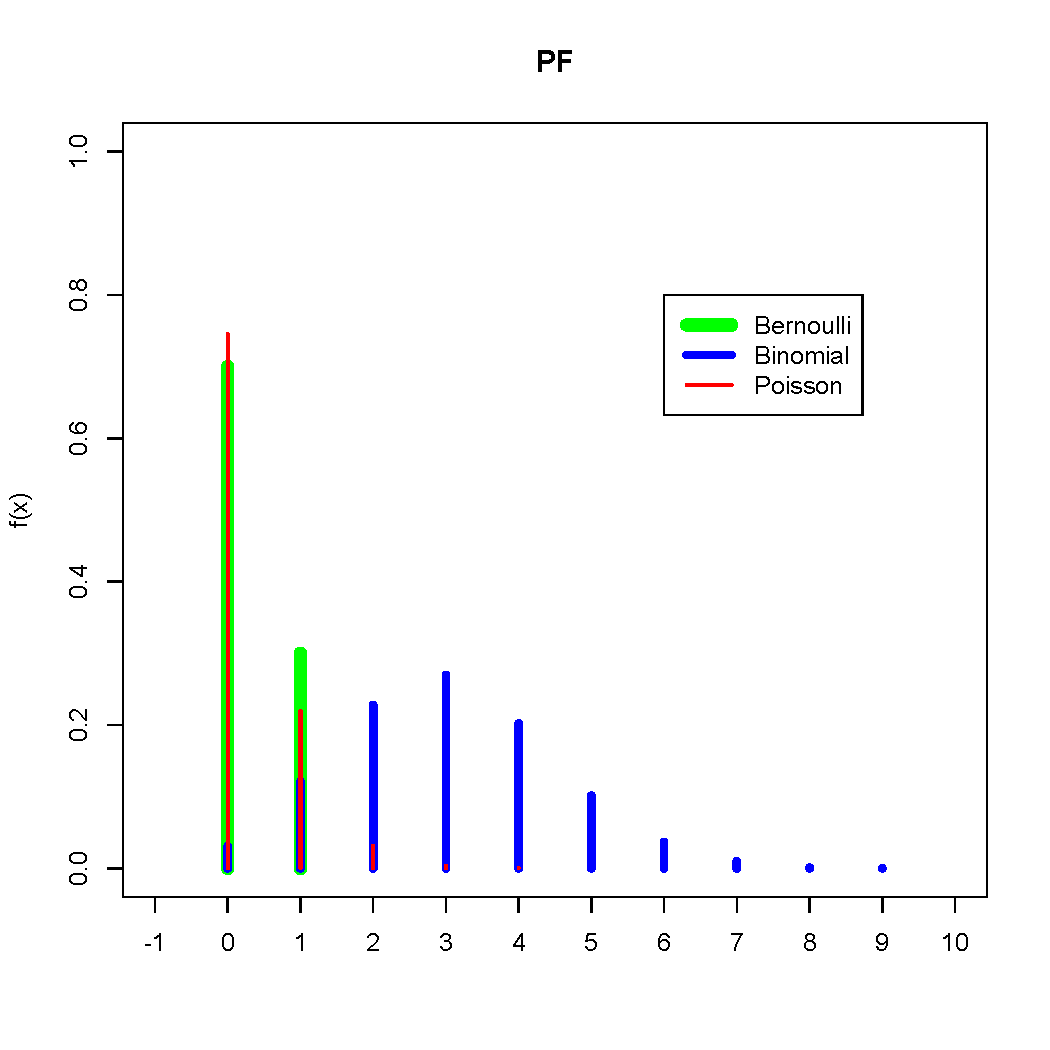
\includegraphics[width= 4 in]{3dists.pdf}

\end{frame}





\begin{frame}{Functions of Random Variables}
\begin{defn}
If $Y=g(X)$, and $X$ is a random variable with probability mass function $p_X(x)$, $Y$ is a random variable with pmf:
  $$p_Y(y)=\sum_{\{x| g(x)=y\}} p_X(x)$$
\end{defn}

\end{frame}






\end{document}